\chapter{Aprendizaje automático}

	\section{Perceptrón}
	
		Ya en el año 1958, el psicólogo Frank Rosenblatt propuso un modelo llamado perceptrón el cual estaba basado en el comportamiento y funcionamiento de las neuronas de un humano, y que podía aprender ponderando cada coeficiente de entrada a la neurona\cite{historiaIA}. Hoy en día, tal y como se mostrará en esta sección, el perceptrón es la unidad fundamental de muchos modelos de \textit{machine learing} y \textit{deep learning}. \\
		
		Como se verá durante esta sección, este modelo ayuda a solucionar problemas de clasificación supervisada. Se dispone de una serie de valores de entrada $x_1, x_2, \hdots, x_n$ y se tiene una serie de valores de salida $y_1, y_2, \hdots, y_m$ que representan a qué clase pertenece la entrada ($2^m$ clases posibles). Esto se consigue mediante la ayuda de sus parámetros, que son una serie de pesos $w_1, w_2, \hdots, w_n$ y un sesgo o \textit{bias} $b$; y sus hiperparámetros, entre los que se encuentra una función $f$ de activación. 
		
		\begin{figure}[!h]
			\centering
			\begin{tikzpicture}
				\foreach \i in {1, 2}
					\pgfmathsetmacro{\resta}{int(\i - 1)}
					\node[circle, draw, fill=gray!20] (x-\i) at (0, -1 * \resta - \resta) {$x_{\i}$};
				\node (dots) at (0, -4) {$\vdots$};
				\node[circle, draw, fill=gray!20] (x-3) at (0, -6) {$x_{n}$};
				\node[circle, draw, fill=gray!20] (n) at (5,-3) {$n_1$};
				\node[circle, draw, fill=gray!20] (a) at (7,-3) {$a_1$};
				\node[circle, draw, fill=gray!20] (b) [below = of n] {$b_1$};
				\node[circle, draw, fill=gray!20] (y) [right = of a] {$y_1$};
				
				\foreach \i in {1, 2}
					\draw[-] (x-\i) -- (n) node [midway, above, sloped] {$w_{\i}$};
				\draw[-] (x-3) -- (n) node [midway, below, sloped] {$w_n$};
				\draw[-] (n) -- (a);
				\draw[-] (a) -- (y);
				\draw[-] (b) -- (n) node [midway, right] {$1$};
			\end{tikzpicture}
			\caption{Arquitectura de un perceptrón}
			\label{fig:perceptron}
		\end{figure}
		
		En la \Cref{fig:perceptron} se muestra la arquitectura del caso más simple de un perceptrón. Se tienen $n$ entradas y una única salida. La primera parte del diagrama representa que tal y como decía Rosenblatt, cada valor de entrada debe multiplicarse por un cierto peso, de tal forma que si se representa esto en función de sus valores en un instante $k$, lo que se computa en el nodo $n_1$ es la siguiente operación. 
		
		$$
		n_1(k) = b_1(k) + \sum_{i=1}^n x_i(k)w_i(k)
		$$
		
		Una vez se ha realizado este cálculo, el valor pasa por una función de activación en el nodo $a_1$, pues esta arquitectura es común utilizarla para clasificar una entrada y es muy útil obtener una salida binaria donde se active únicamente la salida que represente la clase a la que pertenece la entrada dada. Aunque existen diferentes funciones de activación para las neuronas, al trabajar con un perceptrón, la función de activación por excelencia es la función escalón de Heaviside, donde $\mathcal{U}: \mathbb{R} \longrightarrow \{0, 1\}$ y su expresión analítica es
		
		$$
		\mathcal{U}(x) = \left\{\begin{array}{ccc}
			0 & \text{si} & x < 0\\
			1 & \text{si} & x \geq 0
		\end{array}
		\right..
		$$
		
		Combinando ambas expresiones, se puede resumir en que la salida del perceptrón es equivalente a la siguiente ecuación: 
		
		$$
		y_1(k) = \left\{\begin{array}{ccc}
			0 & \text{si} & b_1(k) + \displaystyle\sum_{i=1}^n x_i(k)w_i(k) < 0\\
			1 & \text{si} & b_1(k) + \displaystyle\sum_{i=1}^n x_i(k)w_i(k) \geq 0
		\end{array}
		\right.
		$$
		
		Para dar un ejemplo claro de cómo funciona el perceptrón, se pueden tomar una serie de observaciones que tengan dos valores de entrada y uno de salida. Además, se supondrá que existen dos clases. Esto a fin de cuentas es asignar un valor de 0 o 1 a cada punto de $\mathbb{R}^2$ tal y como se describe en la \Cref{fig:labeled_data}. 
		
		\begin{figure}[!h]
			\centering
			\begin{tikzpicture}
				\begin{axis}[ymin = -2.5, ymax = 2.5, xmax = 2.5, xmin = -2.5, xticklabel = \empty, yticklabel = \empty, minor tick num = 1, axis lines = middle, xlabel = $x$, ylabel = $y$]
					\addplot[only marks, mark = *] coordinates {(1, 2)};
					\addplot[only marks, mark = triangle*] coordinates {(-1, 2) (0, -1)};
				\end{axis}
			\end{tikzpicture}
			\caption{Puntos etiquetados en $\mathbb{R}^2$}
			\label{fig:labeled_data}
		\end{figure}
		
		Una solución rápida sería trazar una recta $r: ax + by + c = 0$ que separe $\mathbb{R}^2$ en dos regiones, de forma que todo punto que pertenezca a una región pertenece entonces a una misma clase, tal y como se observa en la \Cref{fig:separated_label_data}. Esta recta suele llamarse \textit{decision boundary} o frontera de decisión. El problema entonces es hallar la recta $r$, pero se cumple que para este ejemplo es de la forma $w_1 x + w_2 y + b = 0$, siendo el problema encontrar los parámetros adecuados del modelo. La idea puede extrapolarse a diferente tamaño de entrada tomando un hiperplano de la forma $\textbf{w}^t \textbf{x} + b = 0$. \\
		
		Las preguntas a resolver ahora son, ¿existen siempre dichos parámetros? ¿Cómo pueden hallarse? El propio Minsky se hizo estas preguntas en \cite{perceptrons} y se dio cuenta de que dichos parámetros sí pueden hallarse en un número finito de pasos, siempre y cuando los puntos sean linealmente separables. Un ejemplo que no es linealmente separable es el de la función XOR tal y como se muestra en la \Cref{table:xor,fig:xor}, pues no existe una recta $r$ que separe $\mathbb{R}^2$ en dos regiones de tal forma que cada región contenga puntos de una única clase, sería necesaria una frontera de decisión no lineal. 
		
		\begin{figure}
			\centering
			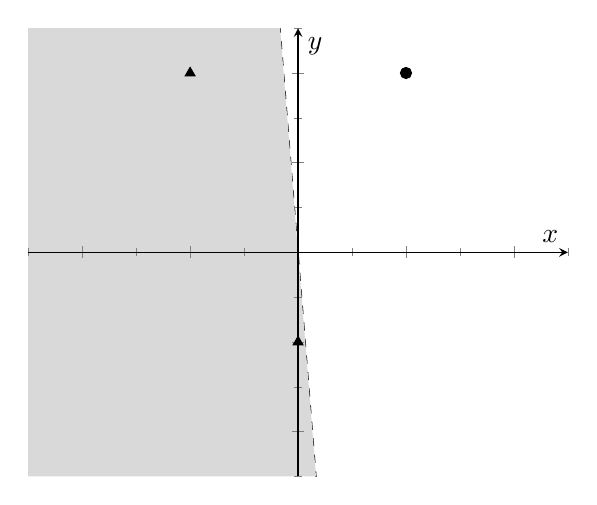
\begin{tikzpicture}
				\begin{axis}[ymin = -2.5, ymax = 2.5, xmax = 2.5, xmin = -2.5, xticklabel = \empty, yticklabel = \empty, minor tick num = 1, axis lines = middle, xlabel = $x$, ylabel = $y$, axis on top]
					\addplot[only marks, mark = *] coordinates {(1, 2)};
					\addplot[only marks, mark = triangle*] coordinates {(-1, 2) (0, -1)};
					\addplot[domain = -3:3, samples = 2, dashed] {-15*x};
					\draw[fill = gray!30, draw = none] (axis cs:-2.5, -2.5) -- (axis cs:-2.5, 2.5) -- (axis cs: -1/6, 2.5) -- (axis cs:1/6, -2.5);
				\end{axis}
			\end{tikzpicture}
			\caption{Puntos separados en $\mathbb{R}^2$}
			\label{fig:separated_label_data}
		\end{figure}
		
		\begin{table}[H]
			\centering
			\begin{tabular}{|c|c|c|}\hline
				$x$ & $y$ & $x \oplus y$\\\hline
				0 & 0 & 0\\\hline
				0 & 1 & 1\\\hline
				1 & 0 & 1\\\hline
				1 & 1 & 0\\\hline
			\end{tabular}
			\caption{Función XOR}
			\label{table:xor}
		\end{table}
		
		\begin{figure}
			\centering
			\begin{tikzpicture}
				\begin{axis}[ymin = -.5, ymax = 2.5, xmax = 2.5, xmin = -.5, xticklabel = \empty, yticklabel = \empty, minor tick num = 1, axis lines = middle, xlabel = $x$, ylabel = $y$]
					\addplot[only marks, mark = *] coordinates {(0, 0) (1, 1)};
					\addplot[only marks, mark = triangle*] coordinates {(0, 1) (1, 0)};
				\end{axis}
			\end{tikzpicture}
			\caption{Valores de $x \oplus y$ en  $\mathbb{R}^2$}
			\label{fig:xor}
		\end{figure}
		
		En cuanto a la pregunta de cómo hallar los parámetros, se consideran las siguientes ecuaciones\cite{nndesign}, donde $\textbf{w}$ es el vector de pesos, $t$ el valor esperado, y $a$ la salida del perceptrón y se aplica el \Cref{algo:perceptron} para obtener los parámetros óptimos. En dicho algoritmo se supondrá que existe una matriz $X$ de $n$ filas que contiene los diferentes $\textbf{x}$. 
		
		\begin{equation}
			\label{eq:perceptron}
			\begin{gathered}
				\textbf{w}(k+1) = \textbf{w}(k) + e(k)\textbf{x}(k)\\
				b(k+1) = b(k) + e(k)\\
				e(k) = t(k) - a(k)\\
				a(k) = \mathcal{U}(\textbf{w}^t(k)\textbf{x}(k))
			\end{gathered}
		\end{equation}
		
		
		\begin{algorithm}
			\SetProgSty{texttt}\DontPrintSemicolon
			
			\caption{Regla de aprendizaje del perceptrón}
			\label{algo:perceptron}
			
			\Datos{$X, \textbf{t}$}
			\Resultado{$\textbf{w}, b$}
			$b \gets 0$\\
			$\textbf{w} \gets$ \texttt{random}\\
			$k \gets 0$\\
			\Repetir{$\lnot$\texttt{acabar}}{
				\texttt{acabar} $\gets$ \texttt{true}\\
				\Para{$i \gets k$ \KwTo $k + n - 1$}{
					$e(i) \gets t(i) - a(i)$\\
					$\textbf{w}(i+1) \gets \textbf{w}(i) + e(i)\textbf{x}(i \pmod n)$\\
					$b(i+1) \gets b(i) + e(i)$\\
					\texttt{acabar} $\gets$ \texttt{acabar} $\land \, e(i) == 0$ 
				}
				$k \gets k + n - 1$
			}
		\end{algorithm}
		
		A cada una de las iteraciones que realiza el bucle exterior se les denomina épocas o \textit{epoch}, que consiste en realizar el proceso de entrenamiento sobre todo el conjunto de datos. En este caso se está suponiendo que no va a recibir casos que no sean linealmente separables, pero de lo contrario se puede añadir un contador \texttt{max\_epochs} y fijar un número máximo para no caer en un bucle infinito. No sería tarea fácil determinar dicho valor, pues aunque el algoritmo converge en los casos previamente explicados, no en todos lo hace de manera rápida. A continuación se muestra cómo obtener una solución para el caso de la \Cref{fig:labeled_data} aplicando el \Cref{algo:perceptron}. 
		
		$$
		X = \begin{pmatrix}
			1 & -1 & 0\\
			2 & 2 & -1
		\end{pmatrix} \,\,\, \textbf{t} = \begin{pmatrix}
		1 & 0 & 0
		\end{pmatrix} \,\,\, \textbf{w}(0) = \begin{pmatrix}
		1\\1 \end{pmatrix} \,\,\, b(0) = 0
		$$
		
		\begin{enumerate}[label = \textbf{\arabic*. }]
			\setcounter{enumi}{-1}
			\item \begin{itemize}
				\item $a(0) = \mathcal{U}(\textbf{w}^t(0)\textbf{x}(0)) = \mathcal{U}\left(\begin{pmatrix}1 & 1\end{pmatrix}\begin{pmatrix}
					1\\2 \end{pmatrix} + 0\right) = 1$
				\item $e(0) = t(0) - a(0) = 1 - 1 = 0$
				\item $\textbf{w}(1) = \textbf{w}(0)$
				\item $b(1) = b(0)$
			\end{itemize}
			
			\item \begin{itemize}
				\item $a(1) = \mathcal{U}(\textbf{w}^t(1)\textbf{x}(1)) = \mathcal{U}\left(\begin{pmatrix}1 & 1\end{pmatrix}\begin{pmatrix}
					-1\\2 \end{pmatrix} + 0\right) = 1$
				\item $e(1) = t(1) - a(1) = 0 - 1 = -1$
				\item $\textbf{w}(2) = \textbf{w}(1) + e(1)\textbf{x}(1) = \begin{pmatrix}1\\ 1\end{pmatrix} - \begin{pmatrix}-1\\2\end{pmatrix} = \begin{pmatrix}2\\ -1\end{pmatrix}$
				\item $b(2) = b(1) + e(1) = -1$
			\end{itemize}
			
			\item \begin{itemize}
				\item $a(2) = \mathcal{U}(\textbf{w}^t(2)\textbf{x}(2)) = \mathcal{U}\left(\begin{pmatrix}2 & -1\end{pmatrix}\begin{pmatrix}
					0\\-1 \end{pmatrix} -1\right) = 1$
				\item $e(2) = t(2) - a(2) = 0 - 1 = -1$
				\item $\textbf{w}(3) = \textbf{w}(2) + e(2)\textbf{x}(2) = \begin{pmatrix}2\\ -1\end{pmatrix} - \begin{pmatrix}0\\-1\end{pmatrix} = \begin{pmatrix}2\\ 0\end{pmatrix}$
				\item $b(3) = b(2) + e(2) = -2$
				\item $\texttt{acabar} = \texttt{true} \land \texttt{false} \land \texttt{false} = \texttt{false}$
			\end{itemize}
			
			\item \begin{itemize}
				\item $a(3) = \mathcal{U}(\textbf{w}^t(3)\textbf{x}(3\pmod{3})) = \mathcal{U}\left(\begin{pmatrix}2 & 0\end{pmatrix}\begin{pmatrix}
					1\\2 \end{pmatrix} -2\right) = 1$
				\item $e(3) = t(3) - a(3) = 1 - 1 = 0$
				\item $\textbf{w}(4) = \textbf{w}(3)$
				\item $b(4) = b(3)$
			\end{itemize}
			
			\item \begin{itemize}
				\item $a(4) = \mathcal{U}(\textbf{w}^t(4)\textbf{x}(4\pmod{3})) = \mathcal{U}\left(\begin{pmatrix}2 & 0\end{pmatrix}\begin{pmatrix}
					-1\\2 \end{pmatrix} -2\right) = 0$
				\item $e(4) = t(4) - a(4) = 0 - 0 = 0$
				\item $\textbf{w}(5) = \textbf{w}(4)$
				\item $b(5) = b(4)$
			\end{itemize}
			
			\item \begin{itemize}
				\item $a(5) = \mathcal{U}(\textbf{w}^t(5)\textbf{x}(5\pmod{3})) = \mathcal{U}\left(\begin{pmatrix}2 & 0\end{pmatrix}\begin{pmatrix}
					0\\-1 \end{pmatrix} -2\right) = 0$
				\item $e(5) = t(5) - a(5) = 0 - 0 = 0$
				\item $\textbf{w}(6) = \textbf{w}(5)$
				\item $b(6) = b(5)$
				\item $\texttt{acabar} = \texttt{true} \land \texttt{true} \land \texttt{true} = \texttt{true}$
			\end{itemize}
		\end{enumerate}
		
		La ejecución del algoritmo finaliza tras dos épocas, donde en la primera de ellas va ajustando los pesos y el sesgo de manera adecuada, y en la segunda verifica que todas las observaciones han sido clasificadas de manera correcta. La frontera de decisión obtenida es la recta $r: 2x - 2 = 0$, que es una recta vertical. Una observación a realizar es que $\textbf{x}(1) \in r$, por tanto ¿a qué clase pertenece? Esto depende de la función de transferencia empleada, al utilizar $\mathcal{U}$ la clasificación es correcta, pero al cambiarla por otra, podría no serlo y necesitaría de más épocas para realizar correctamente la clasificación. \\
		
		La última cuestión que queda por tratar respecto al perceptrón es el porqué se verifica que en el caso de que los puntos dados sean linealmente separables, en un número finito de pasos, el \Cref{algo:perceptron} terminará su ejecución y con el $\textbf{w}$ óptimo, tal y como se enunciaba en el \textbf{Teorema de Convergencia del Perceptrón}. A continuación se realiza su demostración basándose en la que se encuentra en \cite{nndesign} pero de forma más clara y simple. Para comenzar con la demostración será necesario definir una serie de elementos, comenzando por $\Omega(k)$ y $\textbf{z}(k)$. Se entiende que se están concatenando vectores, no definiendo ``vectores dentro de vectores''. 
		
		$$
		\Omega(k) = \begin{pmatrix}
			\textbf{w}(k)\\
			b(k)
		\end{pmatrix} \,\,\, \textbf{z}(k) = \begin{pmatrix}
		\textbf{x}(k)\\
		1
		\end{pmatrix}
		 \,\,\, \Omega(0) = \begin{pmatrix}
			0\\0\\\vdots\\0
		\end{pmatrix}
		$$
		
		Con estos elementos y el cálculo de $a(k)$ en la \Cref{eq:perceptron} es fácil ver que $n(k) = \Omega^t(k)\textbf{z}(k)$. Recordando los posibles valores de $t(k)$, se deseaba que si dicho valor era 1, entonces $n(k) \geq 0$; y en caso de que valiese 0 entonces se deseaba tener $n(k) < 0$, en resumen, que $t(k) - a(k) = 0$. Otra forma de ver esto es afirmar que en el caso en que $t(k) \neq a(k)$, entonces $\Omega(k)$ debe actualizarse de acuerdo a la \Cref{eq:perceptron}. De esta forma $\Omega(k + 1) = \Omega(k) + e(k)\textbf{z}(k)$. Ahora se considerará la existencia de un vector $\Omega^*$ tal que 
		
		$$
		\forall k \,\, \mathcal{U}(\Omega^{*^t}\textbf{z}(k)) = t(k),
		$$
		
		\noindent es decir, $\Omega^*$ es el vector de pesos óptimo. Además, por comodidad se normalizarán todas las distancias del problema, de manera que $\|\Omega^{*}\| = 1$ y $\|\textbf{z}(k)\| \leq 1$. El último elemento a considerar será $\delta$, que será definido como
		
		$$
		\delta = \min\lbrace\Omega^{*^t}\textbf{z}(i)\rbrace, 
		$$
		
		\noindent tomando además que $\delta > 0$ pues otra manera de definirlo es la distancia al punto más cercano a la frontera de decisión óptima. Con estos elementos se puede comenzar la demostración. Como la regla de actualización es $\Omega(k + 1) = \Omega(k) + e(k)\textbf{z}(k)$, al vector de pesos en un determinado instante (clasificación fallida) se le suma o resta $\textbf{z}(k)$ y a priori no se sabe cuántas veces se va a repetir esto, por lo que la idea de la demostración será ver si la norma del vector de pesos tiene una cota superior e inferior, es decir, se para de sumar o restar otros vectores $\textbf{z}(i)$, de manera que el algoritmo terminaría. Para obtener esto basta con comparar el comportamiento de $\Omega^t(k) \Omega^*$ frente a $\Omega^t(k)\Omega(k)$ (es decir, $\|\Omega\|^2$). \\
		
		Con el primero de los términos, al tratar de corregir un error se verifica que
		
		$$
		\Omega^t(k+1)\Omega^* = (\Omega(k) + e(k)\textbf{z}(k))^t \Omega^* = \Omega^t(k)\Omega^* + e(k)\Omega^{*^t}\textbf{z}(k). 
		$$
		
		Además, por la manera en la que se ha definido $\delta$, el segundo sumando queda ubicado entre $\delta$ y $-\delta$, pudiendo deducir la siguiente desigualdad, por lo que en una actualización el término sólo varía en como máximo $\delta$ unidades.  
		
		\begin{equation}
			\label{eq:inf_delta}
			\Omega^t(k+1)\Omega^* \leq \Omega^t(k)\Omega^* + \delta
		\end{equation}
		
		De la misma manera que se ha analizado el comportamiento de $\Omega^t(k) \Omega^*$ se procede con la actualización de $\Omega^t(k)\Omega(k)$. 
		
		\begin{align*}
			\Omega^t(k+1)\Omega(k+1) &= (\Omega(k) + e(k)\textbf{z}(k))^t(\Omega(k) + e(k)\textbf{z}(k))\\
			&= \Omega^2(k) + (e(k)\textbf{z}(k))^2 + 2e(k)\Omega^t(k)\textbf{z}(k)\\
			&= \Omega^t(k)\Omega(k) + e^2(k)\textbf{z}^t(k)\textbf{z}(k) + 2e(k)\Omega^t(k)\textbf{z}(k)\\
			&= \Omega^t(k)\Omega(k) + e^2(k)\textbf{z}^t(k)\textbf{z}(k) + 2e(k)n(k)
		\end{align*}
		
		En el segundo sumando se tiene que siempre será menor o igual que 1, pues por definición $0 \leq \textbf{z}^t(k)\textbf{z}(k) = \|\textbf{z}(k)\|^2 \leq 1$. Además, el tercer sumando siempre será cero o negativo, pues en todos los casos posibles en los que $e(k) \neq 0$ se cumple que $e(k)n(k) < 0$: 
		
		\begin{itemize}
			\item Si $t(k) = 1 \land n(k) < 0$, entonces $a(k) = 0 \land e(k) > 0$
			\item Si $t(k) = 0 \land n(k) \geq 0$, entonces $a(k) = 1 \land e(k) < 0$
		\end{itemize}
		
		De esta situación se puede deducir la siguiente desigualdad, por lo que en una actualización el término sólo varía en como máximo una unidad.   
		
		\begin{equation}
			\label{eq:sup_delta}
			\Omega^t(k+1)\Omega(k+1) \leq \Omega^t(k)\Omega(k) + 1
		\end{equation}
		
		Una vez se ha observado cómo varían estos términos al actualizarlos, se puede observar qué pasaría con ellos al hacer $m$ actualizaciones. Con el resultado obtenido en las \Cref{eq:inf_delta,eq:sup_delta} se pueden deducir las desigualdades $\delta m \leq \Omega^t(m)\Omega^*$ y $\Omega^t(m)\Omega(m) < m$. \\
		
		Ahora al aplicar la desigualdad de Cauchy--Schwarz\footnote{Esta desigualdad afirma que $\|\textbf{u}\textbf{v}\| \leq \|\textbf{u}\|\|\textbf{v}\|$. }, el valor de $\|\Omega^*\|$, y la propiedad transitiva, se obtiene una cota superior y otra inferior (ambas recuadradas) para $\|\Omega^t(m)\|$, lo que demuestra que el número de actualizaciones es finito y que por tanto el algoritmo converge. 
		
		\begin{align*}
			\boxed{\delta m} &\leq \Omega^t(m)\Omega^* = \|\Omega^t(m)\Omega^*\|\\
			&\leq \|\Omega^t(m)\| \|\Omega^*\| = \|\Omega^t(m)\| = \sqrt{\Omega^t(m)\Omega(m)}\\
			& \leq \boxed{\sqrt{m}} 
		\end{align*}
		
		$$
		\pushQED{\qed} 
		\delta m \leq \|\Omega(m)\| \leq \sqrt{m} \,\,\, \Longrightarrow \,\,\, m \leq \frac{1}{\delta^2}\qedhere
		\popQED
		$$ 
		